\documentclass[10pt,a4paper]{article}

\usepackage[utf8]{inputenc}
\usepackage[T1]{fontenc}
\usepackage[english]{babel}
\usepackage[a4paper,margin=2cm]{geometry}
\setlength{\parskip}{2pt}
\usepackage{graphicx}
\usepackage{float}
\usepackage{caption}
\usepackage{hyperref}
\usepackage{xcolor}
\usepackage{listings}
\usepackage{booktabs}
\usepackage{longtable}
\usepackage{array}
\usepackage{enumitem}
\usepackage{titling}

\hypersetup{
  colorlinks=true, linkcolor=blue!60!black, urlcolor=blue!60!black, citecolor=blue!60!black
}

\definecolor{codegray}{rgb}{0.95,0.95,0.95}
\definecolor{codekey}{rgb}{0.0,0.3,0.7}
\definecolor{codestr}{rgb}{0.6,0.1,0.1}
\definecolor{codecom}{rgb}{0.3,0.5,0.3}

\lstset{
  basicstyle=\ttfamily\footnotesize,
  backgroundcolor=\color{codegray},
  keywordstyle=\color{codekey}\bfseries,
  stringstyle=\color{codestr},
  commentstyle=\color{codecom}\itshape,
  showstringspaces=false,
  breaklines=true,
  frame=single,
  numbers=left, numberstyle=\tiny\color{gray}, numbersep=6pt,
  captionpos=b, tabsize=2
}

\title{\textbf{Plataforma Distribu\'\i da para Acompanhamento\\ de Manuten\c{c}\~ao Veicular com RabbitMQ}}
\author{Grupo XX --- XRSC09 Sistemas Distribu\'\i dos\\
\textit{Membro~1, Membro~2, Membro~3, Membro~4, Membro~5}}
\date{Junho de 2026}

\begin{document}
\maketitle

\begin{abstract}
\noindent Este trabalho apresenta o projeto e o prot\'otipo de uma plataforma distribu\'\i da para acompanhamento em tempo real do servi\c{c}o de manuten\c{c}\~ao veicular, com foco em transpar\^encia ao cliente. A solu\c{c}\~ao adota arquitetura h\'\i brida \emph{edge-cloud} orientada a eventos, usando RabbitMQ como barramento de mensageria, PostgreSQL para metadados e armazenamento local para v\'\i deos. A apresenta\c{c}\~ao discute requisitos, modelo C4 nos n\'\i veis de contexto, containers e componentes, m\'aquina de estados das etapas da ordem de servi\c{c}o, fluxo de mensagens entre cliente, mec\^anico, broker e workers especializados, al\'em do prot\'otipo implementado com Next.js, Express, PostgreSQL e quatro workers Node.js consumindo cinco \emph{exchanges} distintas. Os cen\'arios de avalia\c{c}\~ao mostram que o desacoplamento via mensageria viabiliza escalabilidade horizontal independente para cada tipo de tarefa ass\'\i ncrona e mant\'em a oficina operacional mesmo durante quedas tempor\'arias de conectividade.

\medskip
\noindent\textbf{Palavras-chave:} sistemas distribu\'\i dos; RabbitMQ; AMQP; arquitetura orientada a eventos; \emph{edge computing}; manuten\c{c}\~ao veicular.
\end{abstract}

\section{Introdu\c{c}\~ao}

A confian\c{c}a entre cliente e oficina mec\^anica \'e historicamente fr\'agil. O cliente entrega o ve\'\i culo e raramente acompanha o que foi efetivamente executado, quais pe\c{c}as foram substitu\'\i das, o estado do ve\'\i culo durante o diagn\'ostico e a justificativa dos itens cobrados no or\c{c}amento. Esse desconhecimento gera percep\c{c}\~ao de assimetria, reclama\c{c}\~oes p\'os-servi\c{c}o e perda de fideliza\c{c}\~ao. Empresas que prestam servi\c{c}os de manuten\c{c}\~ao veicular t\^em buscado inovar nesse aspecto, expondo ao cliente final evid\^encias verific\'aveis de cada etapa do reparo.

Este projeto trata o problema como o desenho de um sistema distribu\'\i do completo. Uma oficina moderna possui m\'ultiplos gal\-p\~oes, c\^ameras IP, tablets para mec\^anicos, estoque informatizado e atendimento na recep\c{c}\~ao. O ac\'umulo de dados gerados localmente \(textemdash\) v\'\i deos, fotos, registros de etapas, movimenta\c{c}\~oes de pe\c{c}as, mensagens \(textemdash\) precisa atravessar o lim\-iar entre a oficina e a infraestrutura de nuvem para que o cliente, em qualquer lugar, acompanhe o servi\c{c}o em tempo \emph{quase} real. Essa propaga\c{c}\~ao precisa ser confi\'avel, escal\'avel, tolerante a falhas de rede e capaz de envolver m\'ultiplos servi\c{c}os especializados (processamento de m\'\i dia, controle de estoque, gera\c{c}\~ao de notifica\c{c}\~oes, trilhas de auditoria e relat\'orios).

A motiva\c{c}\~ao para uma abordagem distribu\'\i da \'e direta. A solu\c{c}\~ao monol\'\i tica n\~ao se sustenta: mesmo que tecnicamente vi\'avel, ela acopla rigidamente fun\c{c}\~oes que t\^em perfis de carga muito diferentes. Processar um v\'\i deo de 200~MB \'e barato em paraleliza\c{c}\~ao, custoso em CPU, e n\~ao pode bloquear a resposta s\'\i ncrona da API quando o mec\^anico clica em ``enviar evid\^encia''. Notificar o cliente exige integra\c{c}\~ao com gateways externos (e-mail, SMS, WhatsApp) que falham, demoram e mudam com o tempo. Controlar pe\c{c}as exige isolamento transacional do estoque. Audit\'a-las exige persistir tudo que circula sem mexer no fluxo principal. Cada um desses servi\c{c}os tem cad\^encia, escalabilidade e modo de falha pr\'oprios. Tratar tudo separadamente, sob um barramento de eventos comum, \'e o que permite escalar horizontalmente sem reescrever o n\'ucleo do sistema.

O objetivo geral deste projeto \'e \textbf{modelar, prototipar e avaliar uma plataforma distribu\'\i da orientada a eventos para acompanhamento de manuten\c{c}\~ao veicular}, usando RabbitMQ como middleware de mensageria. Como objetivos espec\'\i ficos: (i) projetar a arquitetura completa do sistema considerando contexto, containers e componentes principais (modelo C4); (ii) modelar a comunica\c{c}\~ao entre processos por meio de \emph{Topic Exchanges}, \emph{Fanout}, \emph{Direct}, \emph{Headers Exchanges} e \emph{Dead Letter Exchanges}; (iii) implementar um prot\'otipo funcional com frontend, backend, banco relacional, broker e workers; (iv) avaliar o sistema em cen\'arios de uso end-to-end com m\'ultiplos processos distribu\'\i dos.

\section{Fundamenta\c{c}\~ao Te\'orica}

\subsection{Sistemas distribu\'\i dos e mensageria ass\'\i ncrona}

Um sistema distribu\'\i do \'e composto por processos que executam em m\'aquinas diferentes e comunicam-se por meio de troca de mensagens. Tanenbaum e Van Steen~\cite{tanenbaum2017dist} classificam os modelos de comunica\c{c}\~ao distribu\'\i da em comunica\c{c}\~ao direta (RPC s\'\i ncrono), comunica\c{c}\~ao orientada a mensagens (filas, t\'opicos), comunica\c{c}\~ao orientada a fluxo (\emph{streaming}) e comunica\c{c}\~ao indireta (\emph{publish-subscribe}, mem\'oria compartilhada distribu\'\i da). A escolha do paradigma depende das caracter\'\i sticas n\~ao-funcionais demandadas pelo dom\'\i nio: lat\^encia, vaz\~ao, confiabilidade, acoplamento temporal e espacial entre componentes.

A comunica\c{c}\~ao orientada a mensagens \'e particularmente adequada para fluxos onde produtor e consumidor n\~ao precisam estar simultaneamente ativos, onde a carga \'e n\~ao-uniforme, e onde a mesma informa\c{c}\~ao deve ser tratada por m\'ultiplos consumidores independentes. O padr\~ao \emph{Publish-Subscribe} desacopla os produtores dos consumidores: o produtor publica um evento em um canal nomeado e n\~ao precisa saber quem est\'a inscrito. Isso permite que novos consumidores sejam adicionados sem alterar o produtor, suportando o que Fowler~\cite{fowler2017eda} chama de \emph{Event Notification}, em oposi\c{c}\~ao a chamadas s\'\i ncronas onde o servi\c{c}o A precisa conhecer e estar conectado ao servi\c{c}o B.

\subsection{RabbitMQ e o protocolo AMQP}

O RabbitMQ~\cite{rabbitmq} \'e um \emph{broker} de mensagens implementado em Erlang que serve como refer\^encia da especifica\c{c}\~ao AMQP 0-9-1. O modelo do AMQP organiza-se em torno de tr\^es abstra\c{c}\~oes: \emph{exchanges} (pontos de publica\c{c}\~ao), \emph{queues} (caixas de mensagens) e \emph{bindings} (regras de roteamento que ligam exchanges a queues). O produtor envia mensagens para uma exchange; o RabbitMQ, segundo o tipo da exchange e as \emph{routing keys} ou \emph{headers}, decide para quais filas a mensagem ser\'a entregue.

Existem quatro tipos principais de exchanges. O \emph{Direct Exchange} roteia mensagens cuja routing key seja exatamente igual \`a do binding. O \emph{Topic Exchange} usa padr\~oes com curingas (``\texttt{*}'' para um token, ``\texttt{\#}'' para zero ou mais tokens) sobre routing keys hier\'arquicas. O \emph{Fanout Exchange} ignora a routing key e entrega a todas as filas ligadas, implementando broadcast. O \emph{Headers Exchange} roteia segundo atributos arbitr\'arios da mensagem. A combina\c{c}\~ao desses tipos permite expressar v\'arios padr\~oes de comunica\c{c}\~ao com um \'unico middleware: \emph{Work Queues} (uma fila, m\'ultiplos consumidores em \emph{round-robin}), \emph{Publish-Subscribe} (Fanout), \emph{Routing} (Direct) e \emph{Topic Routing} (Topic).

Recursos adicionais relevantes incluem: \emph{Dead Letter Exchange} (mensagens rejeitadas s\~ao reencaminhadas para retry ou inspe\c{c}\~ao manual); \emph{TTL} de fila e de mensagem; \emph{prefetch} configur\'avel para controle de paralelismo no consumidor; \emph{quorum queues} para alta disponibilidade; e \emph{Federation/Shovel} para replica\c{c}\~ao entre brokers em redes distintas \(textemdash\) recurso decisivo para a estrat\'egia edge-cloud deste projeto.

Em rela\c{c}\~ao a alternativas, o Apache Kafka~\cite{kreps2011kafka} \'e otimizado para alto \emph{throughput} de \emph{stream processing} com particionamento e reten\c{c}\~ao prolongada de eventos, mas tem semantica de filas menos rica que o AMQP. O gRPC \'e voltado a chamadas s\'\i ncronas tipo RPC sobre HTTP/2, sem desacoplamento temporal. Para um sistema que precisa de \emph{event notification} com routing flex\'\i vel, m\'ultiplos workers especializados consumindo a partir do mesmo broker, baixa lat\^encia e taxa moderada, o RabbitMQ oferece o equil\'\i brio adequado.

\subsection{Arquiteturas orientadas a eventos e modelo C4}

A arquitetura orientada a eventos (EDA)~\cite{fowler2017eda,eda2020arch} estrutura o sistema em torno de eventos imut\'aveis que representam fatos do dom\'\i nio. Cada componente publica e consome eventos sem saber quem est\'a do outro lado, comunicando-se atrav\'es do broker. Para descrever a arquitetura, adotamos o modelo C4 proposto por Brown~\cite{brown2018c4}, que organiza diagramas em quatro n\'\i veis hier\'arquicos: contexto (atores e sistemas externos), containers (unidades de implanta\c{c}\~ao independente), componentes (m\'odulos internos a um container) e c\'odigo (detalhe opcional, frequentemente em classes ou pseudo-c\'odigo).

\subsection{Linguagens, bibliotecas e frameworks adotados}

A implementa\c{c}\~ao do prot\'otipo usa Node.js 20 LTS para backend e workers, Express 4 para a API REST, \texttt{amqplib} 0.10 para comunica\c{c}\~ao AMQP com o RabbitMQ, PostgreSQL 16 para metadados (acessado via \texttt{node-postgres}), Multer para upload multipart de arquivos, e Next.js 14 (React 18) para o portal. A orquestra\c{c}\~ao local \'e feita com Docker Compose, conteinerizando os seis servi\c{c}os principais (frontend, backend, postgres, rabbitmq e quatro workers especializados). Essa escolha favorece reprodutibilidade, baixo custo e curva de aprendizagem suave para uso did\'atico.

\section{Metodologia}

\subsection{An\'alise do Problema}
\label{sec:analise}

O cen\'ario adotado foi sorteado para o grupo na disciplina XRSC09: \emph{acompanhamento de manuten\c{c}\~ao de ve\'\i culos}. Uma empresa que presta servi\c{c}os de manuten\c{c}\~ao deseja oferecer ao cliente acompanhamento das etapas do servi\c{c}o em tempo real \(textemdash\) registro do relato, testes de diagn\'ostico, identifica\c{c}\~ao da causa e execu\c{c}\~ao do reparo, incluindo substitui\c{c}\~ao de pe\c{c}as com rastreamento.

\subsubsection*{Requisitos identificados}

A partir desse cen\'ario, identificamos os seguintes requisitos funcionais principais: autentica\c{c}\~ao com quatro perfis (cliente, mec\^anico, gestor, administrador) e controle de acesso por papel; cadastro de ordens de servi\c{c}o (OS) vinculadas a cliente e ve\'\i culo; m\'aquina de estados expl\'\i cita das etapas, com transi\c{c}\~oes validadas; envio e visualiza\c{c}\~ao de evid\^encias em foto e v\'\i deo; rastreamento de pe\c{c}as solicitadas, reservadas e instaladas; or\c{c}amento com aprova\c{c}\~ao do cliente; notifica\c{c}\~oes em tempo real para o cliente a cada mudan\c{c}a de etapa; trilha de auditoria de todas as a\c{c}\~oes relevantes; relat\'orio final do servi\c{c}o.

Os requisitos n\~ao-funcionais s\~ao igualmente importantes. Resili\^encia: a oficina deve continuar operando mesmo durante quedas de internet. Escalabilidade horizontal: cada tipo de tarefa ass\'\i ncrona (processar v\'\i deo, enviar e-mail, atualizar estoque) precisa escalar de forma independente. Desacoplamento: novos consumidores devem poder ser adicionados sem alterar a API. Seguran\c{c}a: autoriza\c{c}\~ao por papel, segredos fora do c\'odigo, prepara\c{c}\~ao para HTTPS.

\subsubsection*{Componentes envolvidos}

Identificamos os seguintes componentes do dom\'\i nio: c\^ameras IP nos galp\~oes; tablets dos mec\^anicos; recep\c{c}\~ao com terminal pr\'oprio; almoxarifado com estoque informatizado; sala do gestor; servidor local de borda (\emph{edge gateway}) com mini-broker, NAS para v\'\i deos brutos e \emph{switch} L2/L3; conex\~ao com a nuvem; backend central na nuvem; PostgreSQL gerenciado; cluster RabbitMQ na nuvem; \emph{storage} S3/R2 para v\'\i deos definitivos; workers especializados em m\'\i dia, notifica\c{c}\~ao, estoque, auditoria, relat\'orios e billing; portal web acessado por todos os atores.

\subsubsection*{Justificativa para solu\c{c}\~ao distribu\'\i da}

Quatro fatores justificam o uso de uma solu\c{c}\~ao distribu\'\i da. (i) \emph{Escala desigual}: processar v\'\i deo n\~ao escala como atender requisi\c{c}\~oes REST. (ii) \emph{Mais de um destinat\'ario por evento}: uma mudan\c{c}a de etapa precisa atualizar o portal do cliente, gerar trilha de auditoria, atualizar dashboards do gestor e potencialmente enviar e-mail. (iii) \emph{Resili\^encia geogr\'afica}: a oficina precisa continuar registrando evid\^encias mesmo offline. (iv) \emph{Extensibilidade}: novos workers (billing, relat\'orio, integra\c{c}\~ao com seguradoras) devem ser plugados sem mexer no n\'ucleo.

\subsubsection*{Cen\'arios de uso principais}
\begin{itemize}[leftmargin=*]
\item \textbf{C1 \(textendash\) Recep\c{c}\~ao do ve\'\i culo:} atendente registra OS, sistema publica \texttt{workorder.opened}, notifica\c{c}\~ao chega ao cliente.
\item \textbf{C2 \(textendash\) Diagn\'ostico com evid\^encia:} mec\^anico envia v\'\i deos do diagn\'ostico, worker processa em segundo plano, cliente visualiza no portal.
\item \textbf{C3 \(textendash\) Solicita\c{c}\~ao e instala\c{c}\~ao de pe\c{c}a:} mec\^anico solicita pe\c{c}a, inventory-worker reserva no estoque, mec\^anico marca como instalada.
\item \textbf{C4 \(textendash\) Aprova\c{c}\~ao do or\c{c}amento:} or\c{c}amento publicado dispara notifica\c{c}\~ao; resposta do cliente avan\c{c}a a m\'aquina de estados; eventos em cascata liberam o reparo.
\item \textbf{C5 \(textendash\) Conclus\~ao:} mec\^anico avan\c{c}a estado para \texttt{CONCLUIDO}; sistema publica \texttt{workorder.completed}; relat\'orio final disponibilizado.
\end{itemize}

\subsection{Modelagem do Sistema}

A arquitetura proposta combina cliente-servidor (frontend e backend via HTTP/REST), camadas (apresenta\c{c}\~ao, aplica\c{c}\~ao, dados), mensageria ass\'\i ncrona (RabbitMQ entre backend e workers) e implanta\c{c}\~ao h\'\i brida edge-cloud (oficina local + nuvem).

\begin{figure}[H]
\centering
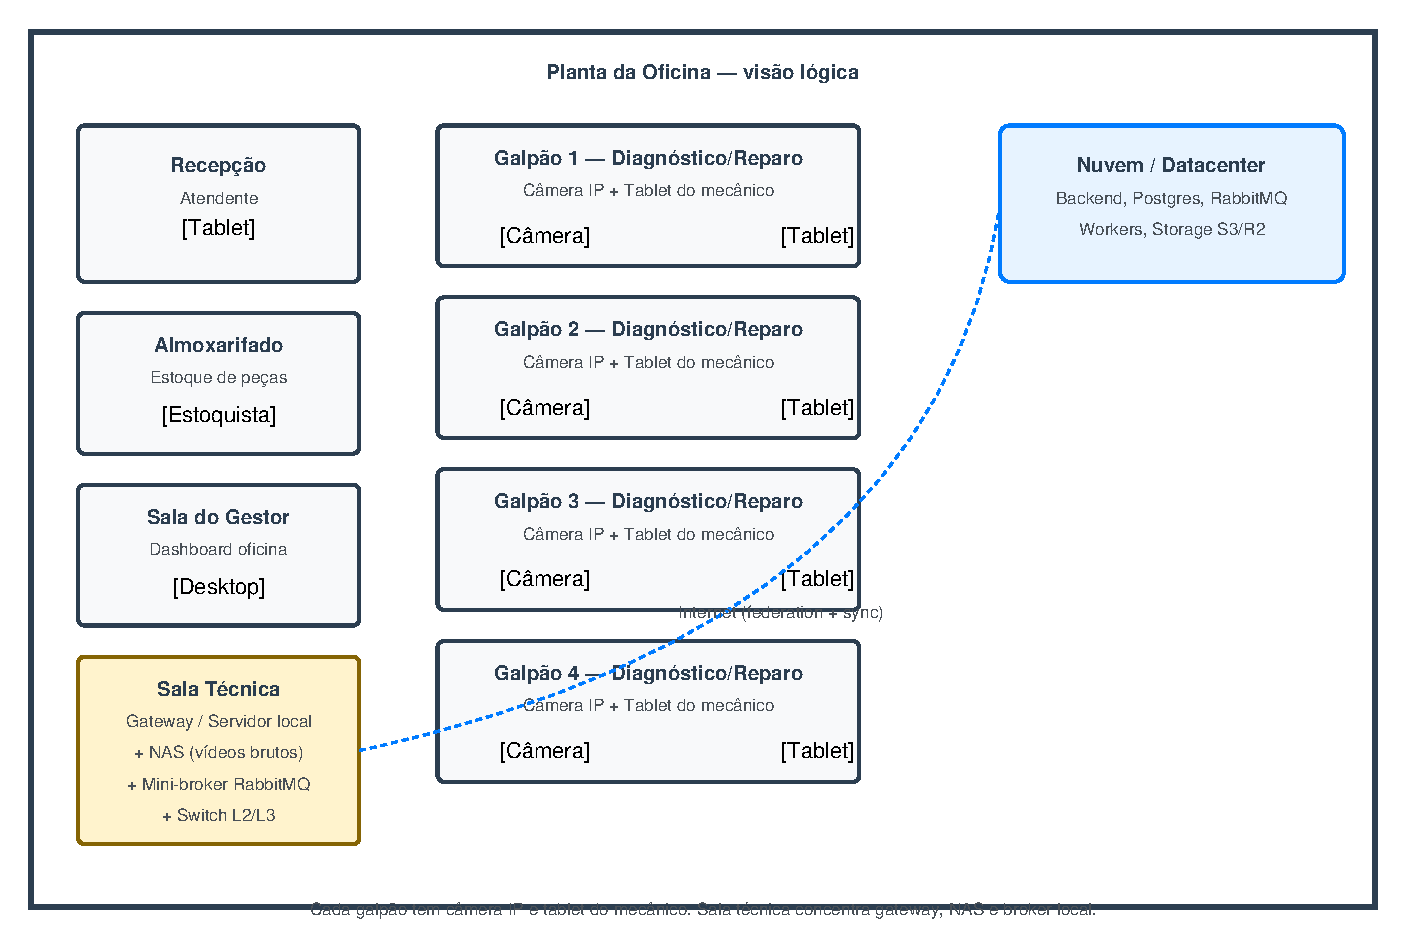
\includegraphics[width=0.65\textwidth]{../diagrams/planta_oficina.pdf}
\caption{Planta l\'ogica da oficina: recep\c{c}\~ao, almoxarifado, sala do gestor, quatro galp\~oes com c\^amera IP e tablet do mec\^anico, e sala t\'ecnica com gateway, NAS e mini-broker RabbitMQ.}
\label{fig:planta}
\end{figure}

\subsubsection*{Modelo C4 \(textendash\) N\'\i vel 1: Contexto}

A Figura~\ref{fig:c4n1} mostra os atores (cliente, mec\^anico, atendente, gestor, administrador) e os sistemas externos (c\^ameras IP, storage S3/R2, gateways email/SMS/WhatsApp, ERP de pe\c{c}as, sistema de pagamento, NF-e). O sistema central concentra a l\'ogica de neg\'ocio e \'e o ponto \'unico de coordena\c{c}\~ao.

\begin{figure}[H]
\centering
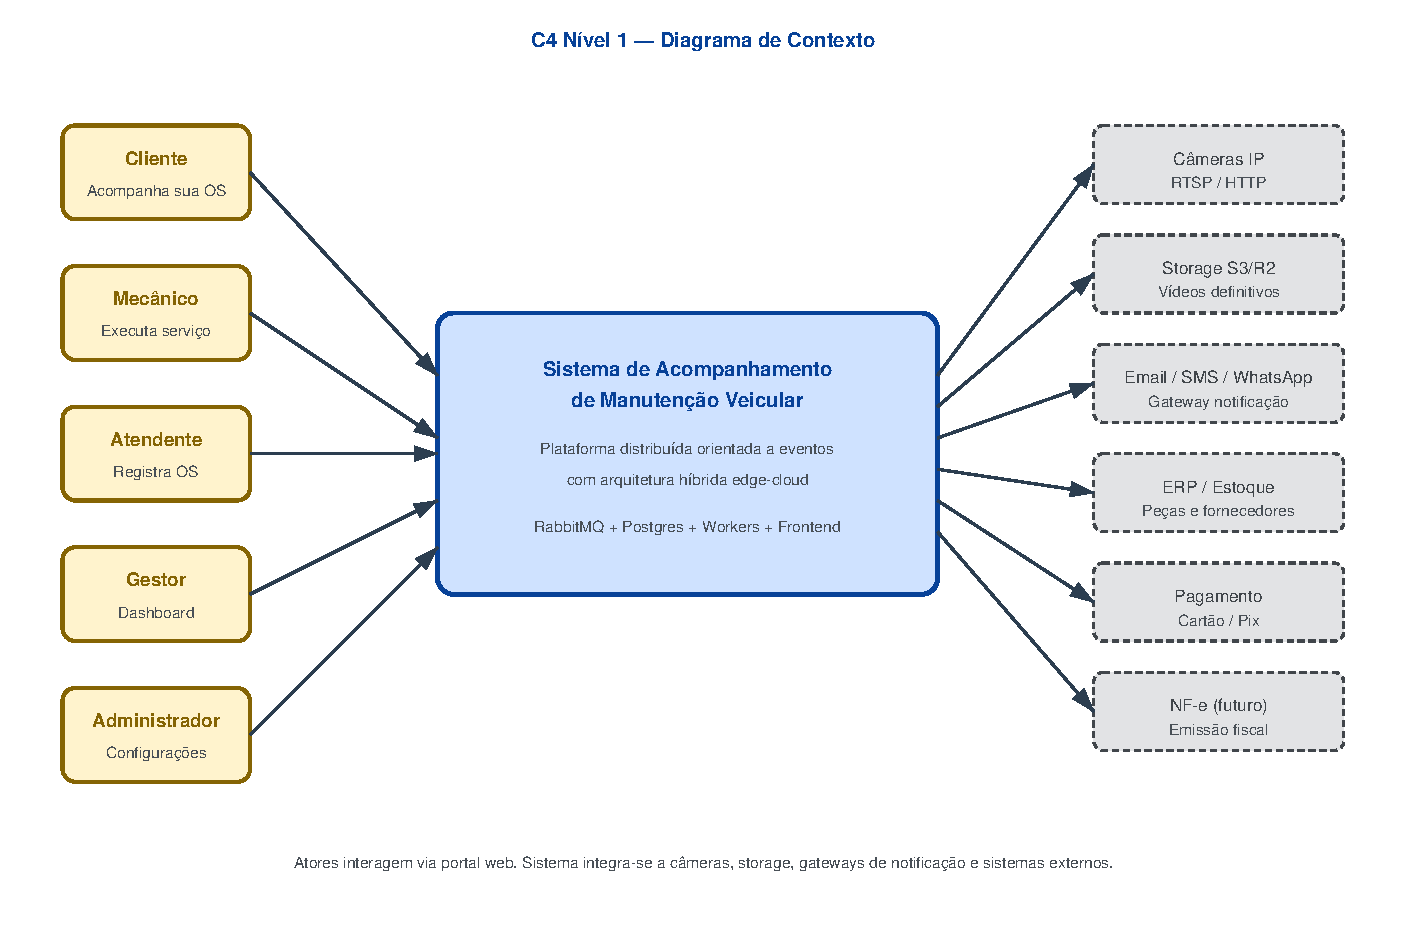
\includegraphics[width=0.65\textwidth]{../diagrams/c4_nivel1_contexto.pdf}
\caption{C4 N\'\i vel 1: diagrama de contexto.}
\label{fig:c4n1}
\end{figure}

\subsubsection*{Modelo C4 \(textendash\) N\'\i vel 2: Containers}

A Figura~\ref{fig:c4n2} detalha os containers organizados em duas zonas: \emph{edge} (oficina) e \emph{cloud} (nuvem). A separa\c{c}\~ao em zonas \'e arquitet\^onica, n\~ao apenas log\'\i stica. Na borda ficam: c\^ameras IP, tablets dos mec\^anicos, terminais da recep\c{c}\~ao e do almoxarifado, \emph{edge gateway} (API local que recebe uploads e armazena temporariamente), \emph{NAS} para v\'\i deos brutos, e mini-broker RabbitMQ federado com o broker da nuvem. Na nuvem ficam: frontend (Next.js), backend (Express), PostgreSQL gerenciado, storage S3/R2 de v\'\i deos definitivos, cluster RabbitMQ e os workers.

\begin{figure}[H]
\centering
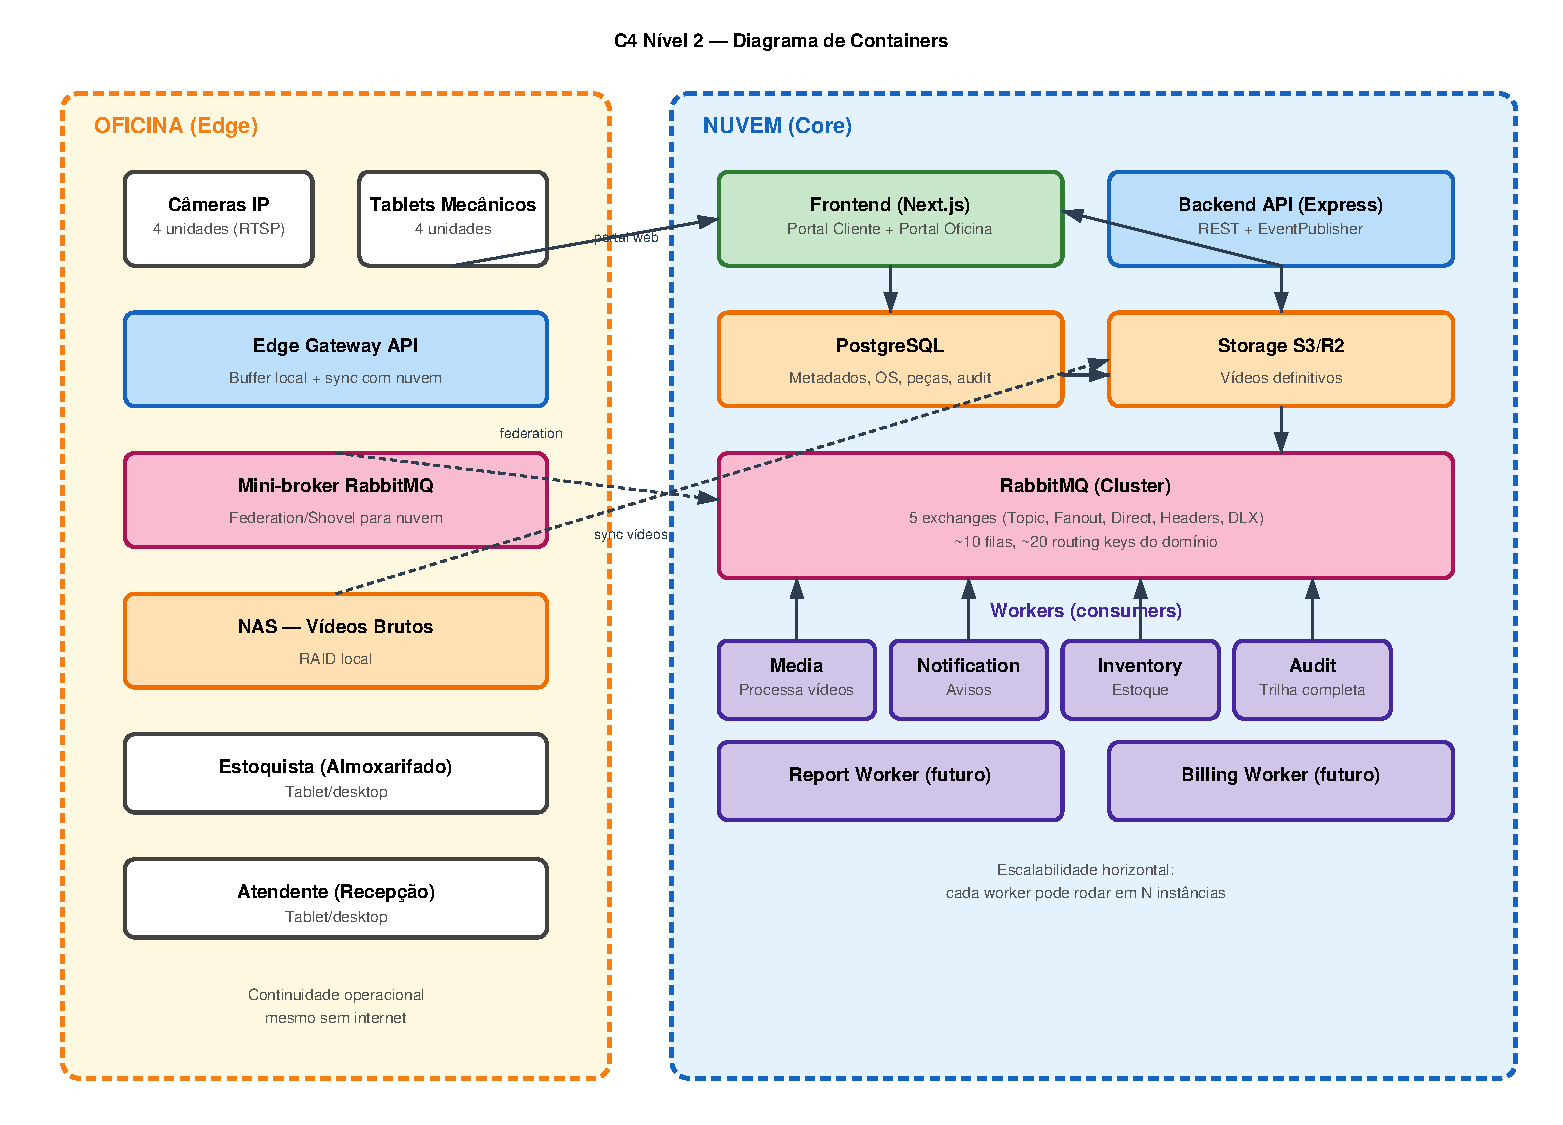
\includegraphics[width=0.72\textwidth]{../diagrams/c4_nivel2_containers.pdf}
\caption{C4 N\'\i vel 2: diagrama de containers edge + cloud.}
\label{fig:c4n2}
\end{figure}

\subsubsection*{Modelo C4 \(textendash\) N\'\i vel 3: Componentes do Backend}

Internamente, o backend organiza-se em controllers (camada de roteamento HTTP), services (l\'ogica de neg\'ocio: \texttt{StepStateMachine}, \texttt{PartService}, \texttt{SessionService}), repositories (acesso a Postgres) e o componente central \texttt{EventPublisher}, que encapsula toda a intera\c{c}\~ao com o broker (Figura~\ref{fig:c4n3}). Esse desenho garante que substituir o middleware no futuro envolva apenas reescrever \texttt{EventPublisher} \(textendash\) o resto do c\'odigo n\~ao conhece o broker.

\begin{figure}[H]
\centering
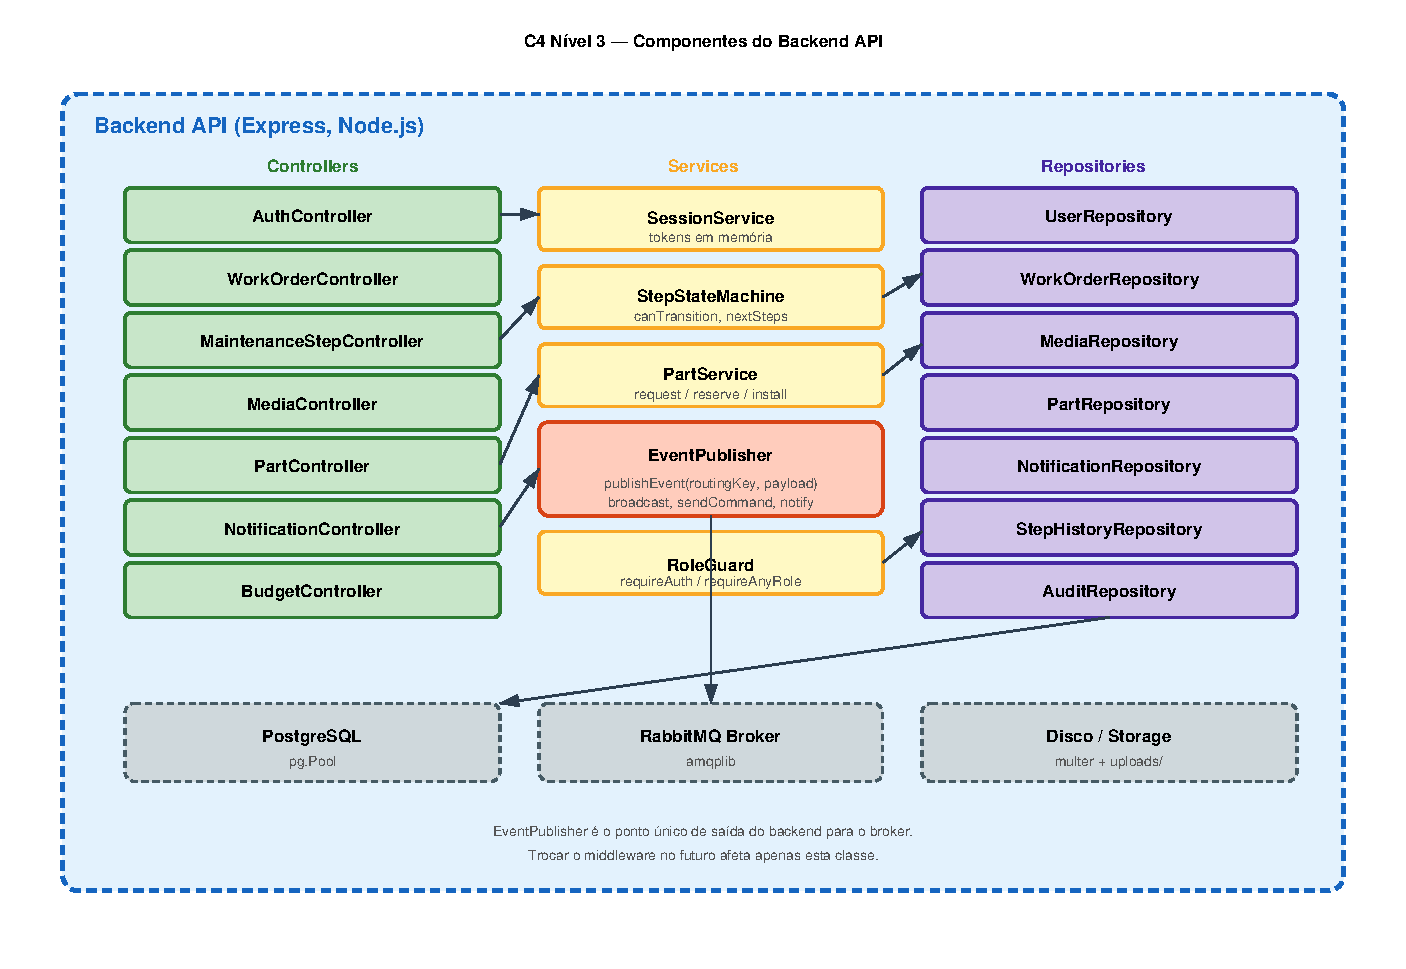
\includegraphics[width=0.72\textwidth]{../diagrams/c4_nivel3_componentes.pdf}
\caption{C4 N\'\i vel 3: componentes internos ao backend.}
\label{fig:c4n3}
\end{figure}

\subsubsection*{M\'aquina de estados das etapas}

A ordem de servi\c{c}o percorre uma sequ\^encia de estados rigidamente validada (Figura~\ref{fig:sm}). Cada transi\c{c}\~ao publica um evento \texttt{maintenance.step.updated} no \emph{Topic Exchange} principal, com \emph{routing key} estruturada como \texttt{maintenance.step.<estado>}. Transi\c{c}\~oes inv\'alidas s\~ao bloqueadas pelo backend com c\'odigo HTTP 409 e a lista de pr\'oximos estados v\'alidos.

\begin{figure}[H]
\centering
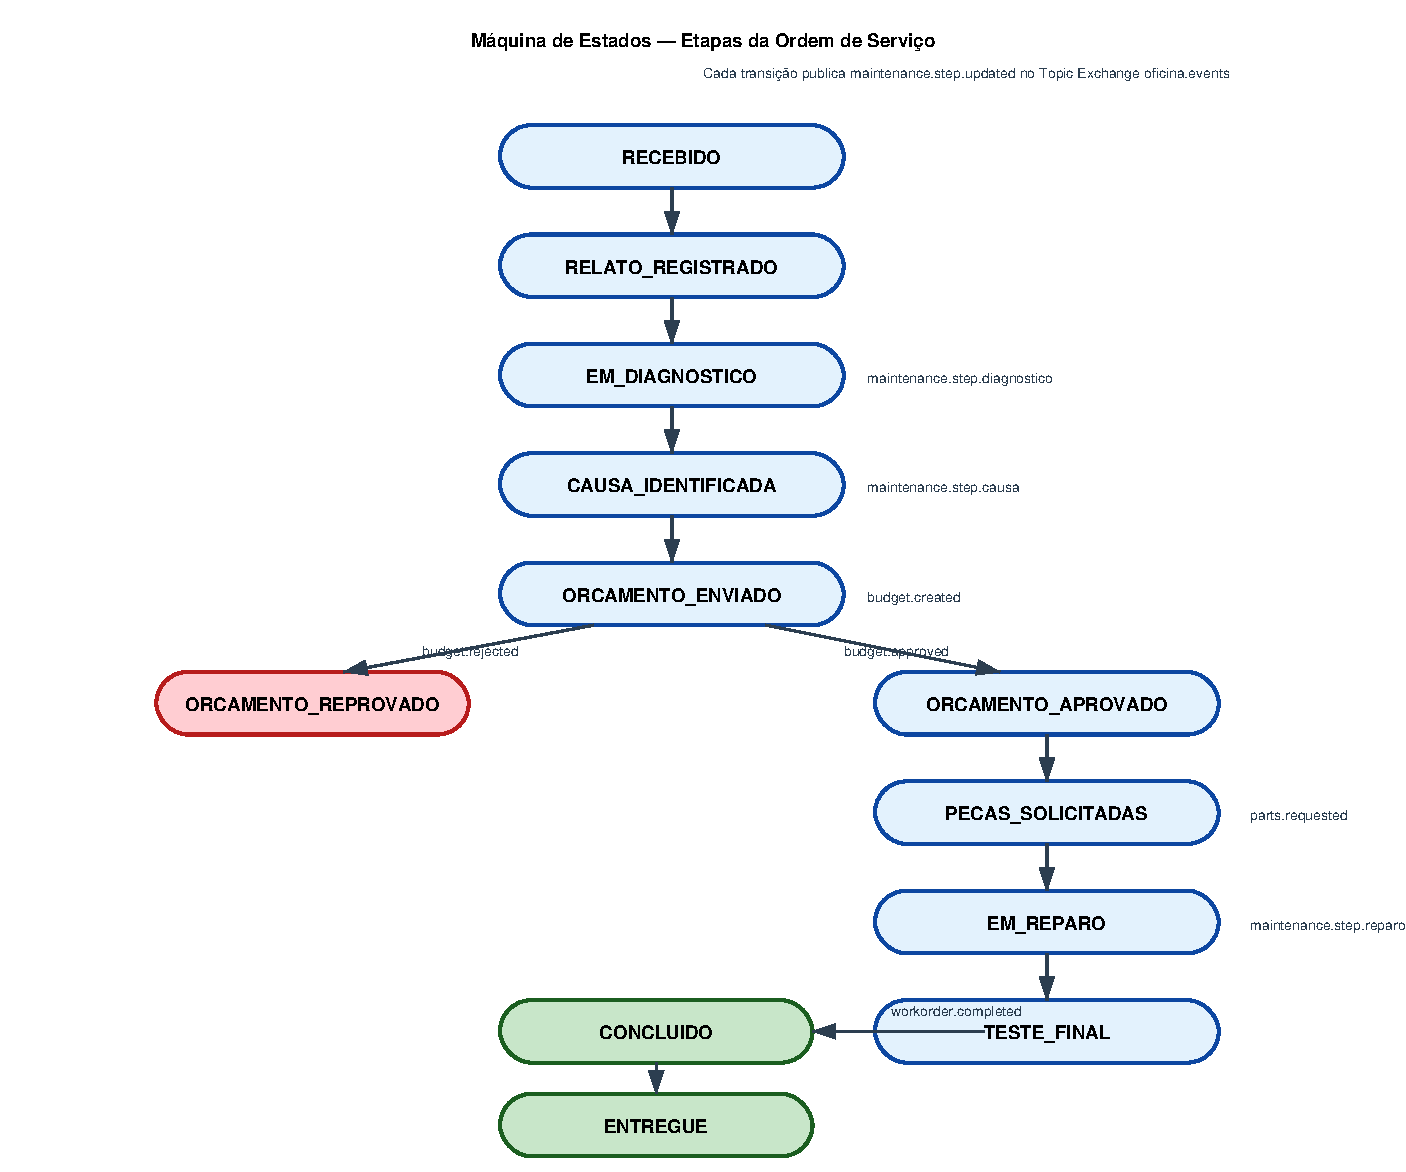
\includegraphics[width=0.55\textwidth]{../diagrams/state_machine.pdf}
\caption{M\'aquina de estados das etapas. Estados terminais em verde; rejei\c{c}\~ao em vermelho.}
\label{fig:sm}
\end{figure}

\subsubsection*{Topologia RabbitMQ}

A Figura~\ref{fig:rabbit} apresenta a topologia completa do broker. S\~ao declaradas cinco exchanges: \texttt{oficina.events} (Topic), \texttt{oficina.broadcast} (Fanout), \texttt{oficina.commands} (Direct), \texttt{oficina.notifications} (Headers), e \texttt{oficina.dlx} (Dead Letter). Cada padr\~ao de comunica\c{c}\~ao distribu\'\i da do AMQP est\'a representado por pelo menos uma exchange. As \emph{routing keys} seguem a conven\c{c}\~ao \texttt{dominio.entidade.acao} (por exemplo, \texttt{parts.requested}, \texttt{budget.approved}, \texttt{media.processed}). A Tabela~\ref{tab:eventos} sumariza o cat\'alogo planejado.

\begin{figure}[H]
\centering
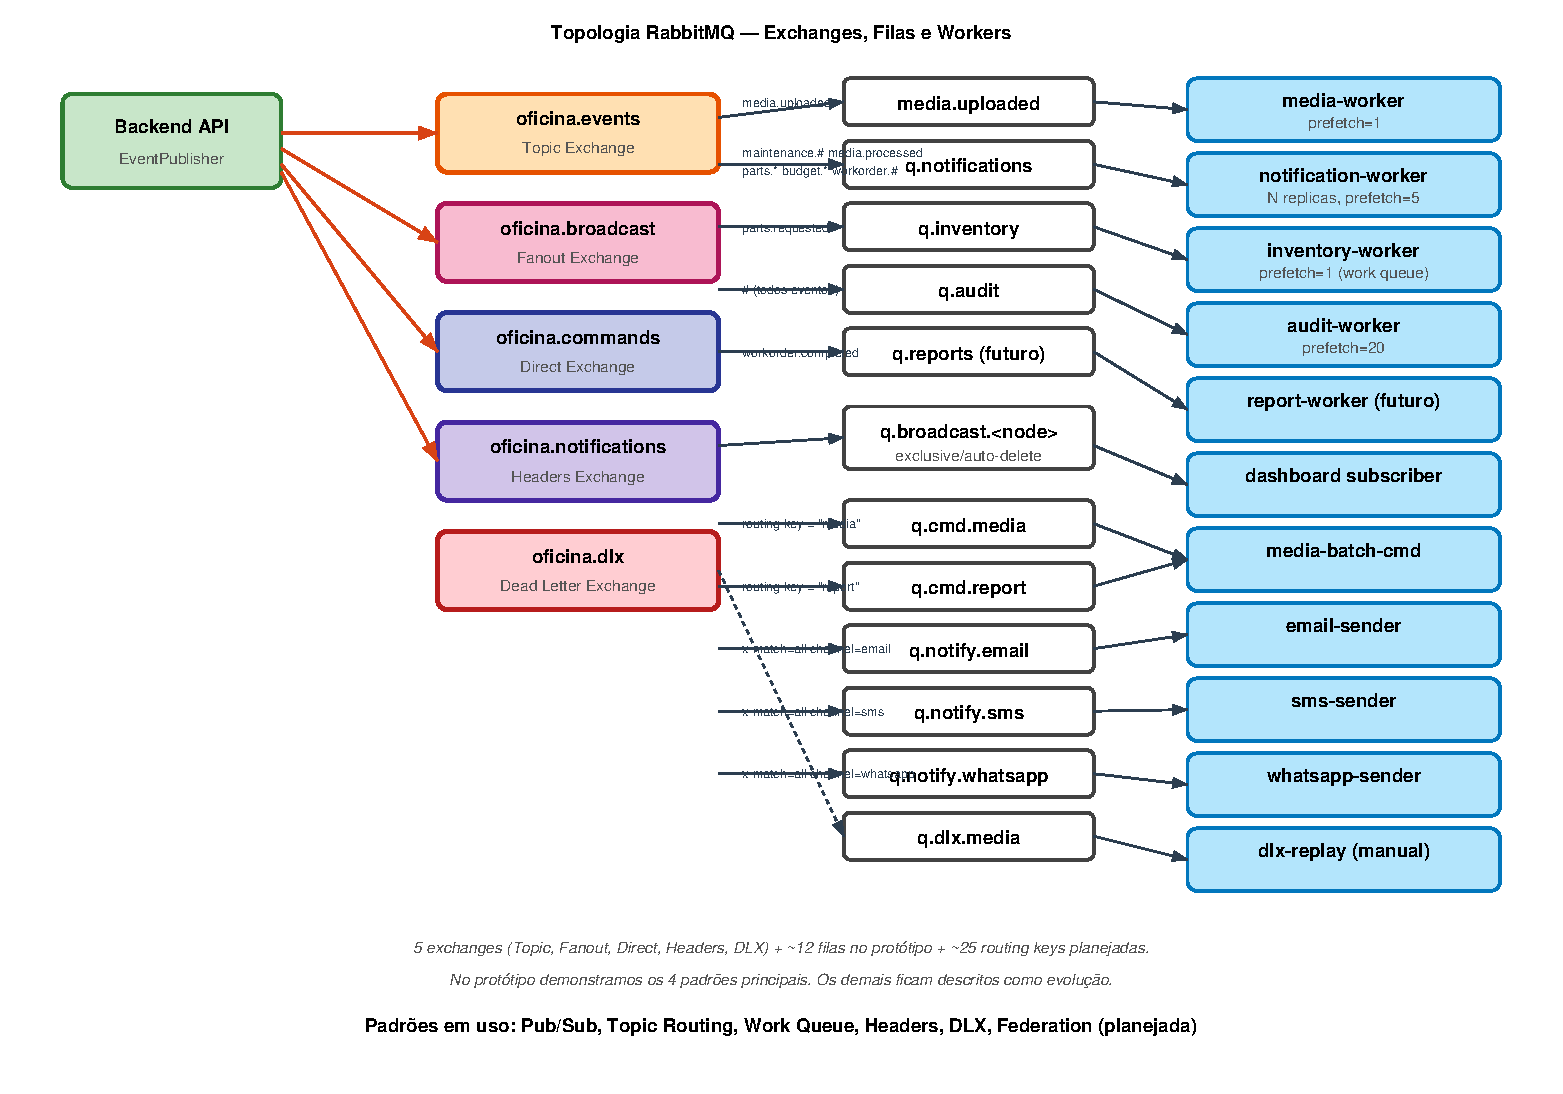
\includegraphics[width=0.72\textwidth]{../diagrams/rabbitmq_topology.pdf}
\caption{Topologia RabbitMQ: exchanges, filas, padr\~oes de bind e workers consumidores.}
\label{fig:rabbit}
\end{figure}

\begin{table}[H]
\centering
\caption{Cat\'alogo de eventos do dom\'\i nio.}
\label{tab:eventos}
\small
\begin{tabular}{@{}llp{6cm}@{}}
\toprule
\textbf{Routing key} & \textbf{Exchange} & \textbf{Quando ocorre} \\
\midrule
\texttt{workorder.opened} & oficina.events & OS \'e aberta pela recep\c{c}\~ao \\
\texttt{maintenance.step.updated} & oficina.events & Mec\^anico avan\c{c}a etapa \\
\texttt{media.uploaded} & oficina.events & Mec\^anico envia foto/v\'\i deo \\
\texttt{media.processed} & oficina.events & Worker conclui processamento \\
\texttt{media.failed} & oficina.dlx & Falha persistente em mensagem \\
\texttt{budget.created} & oficina.events & Or\c{c}amento gerado \\
\texttt{budget.approved} & oficina.events & Cliente aprova or\c{c}amento \\
\texttt{budget.rejected} & oficina.events & Cliente rejeita or\c{c}amento \\
\texttt{parts.requested} & oficina.events & Mec\^anico solicita pe\c{c}a \\
\texttt{parts.reserved} & oficina.events & Pe\c{c}a reservada no estoque \\
\texttt{parts.outofstock} & oficina.events & Pe\c{c}a em falta \\
\texttt{parts.installed} & oficina.events & Pe\c{c}a marcada como instalada \\
\texttt{workorder.completed} & oficina.events & Servi\c{c}o conclu\'\i do \\
\texttt{broadcast.\#} & oficina.broadcast & Avisos globais (manuten\c{c}\~ao, alarmes) \\
\texttt{cmd.<target>} & oficina.commands & Comandos diretos a workers espec\'\i ficos \\
\bottomrule
\end{tabular}
\end{table}

\subsubsection*{Fluxos de mensagem}

A Figura~\ref{fig:seq-midia} ilustra o ciclo do upload de m\'\i dia. O mec\^anico submete arquivos via portal; o backend persiste metadados, publica \texttt{media.uploaded}, e responde imediatamente ao usu\'ario com status \texttt{UPLOADED}. O \texttt{media-worker} consome a mensagem, simula processamento (em produ\c{c}\~ao seria FFmpeg para gera\c{c}\~ao de \emph{thumbnail} e transcodifica\c{c}\~ao), e atualiza o status para \texttt{PROCESSED}, publicando \texttt{media.processed}.

\begin{figure}[H]
\centering
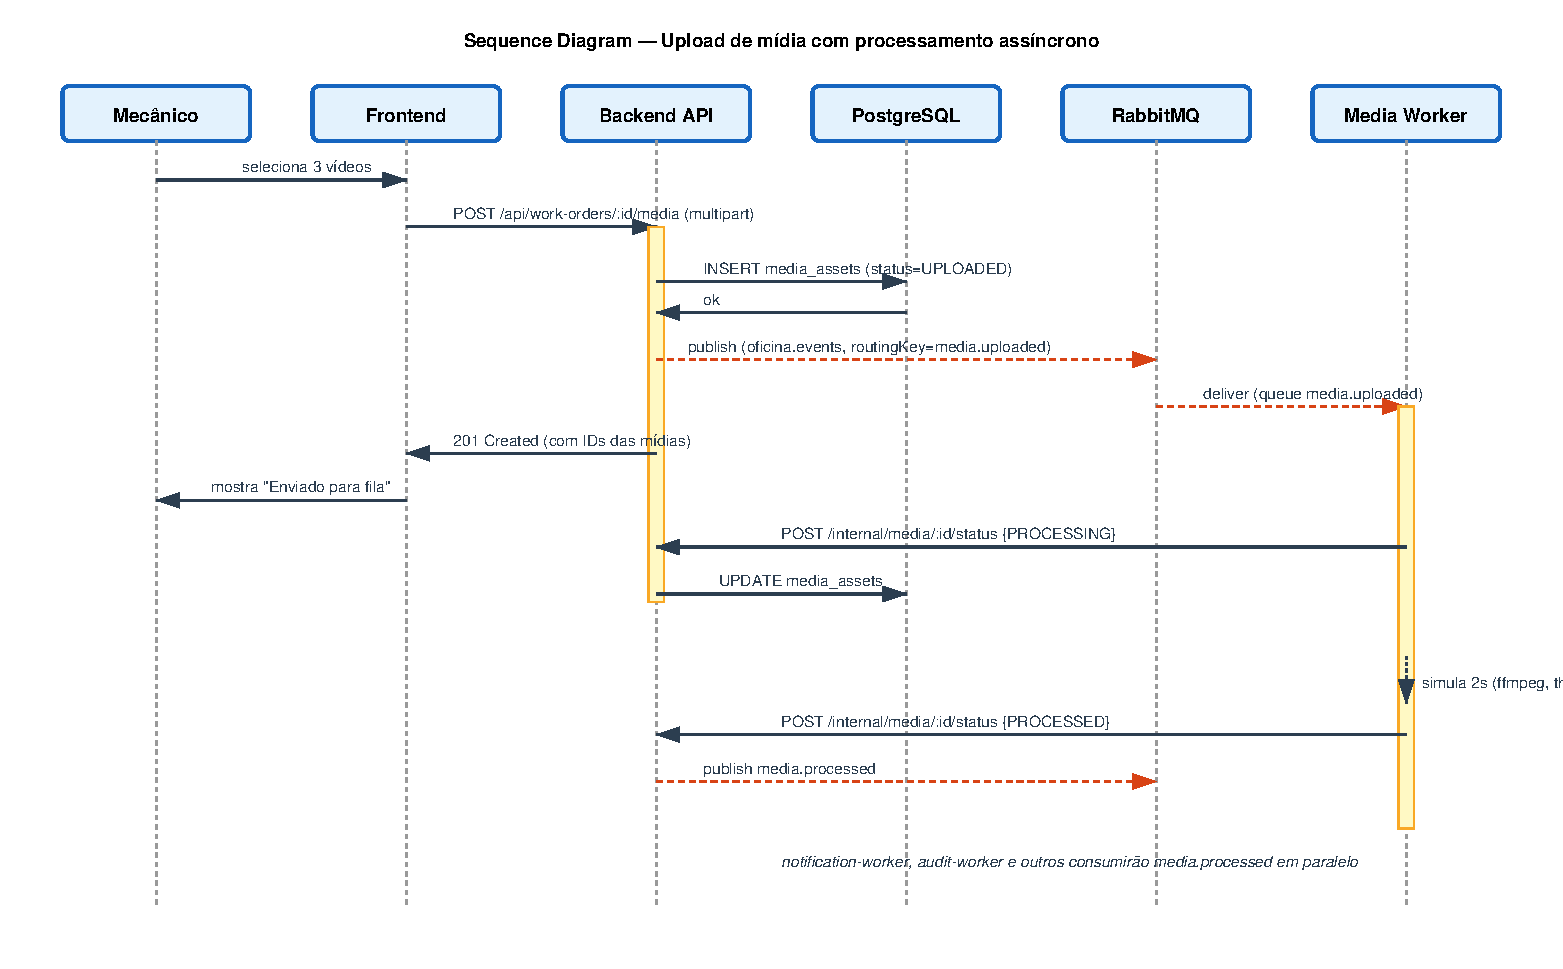
\includegraphics[width=0.72\textwidth]{../diagrams/sequence_midia.pdf}
\caption{Sequence diagram: upload de m\'\i dia e processamento ass\'\i ncrono.}
\label{fig:seq-midia}
\end{figure}

A Figura~\ref{fig:seq-etapa} mostra uma mudan\c{c}a de etapa e a \emph{cascata} de eventos resultante. Uma \'unica chamada de API dispara processamento paralelo em v\'arios workers: o \texttt{notification-worker} cria registros de notifica\c{c}\~ao para os \emph{stakeholders}; o \texttt{audit-worker} grava a entrada na trilha de auditoria; outros workers (relat\'orio, billing) podem ser plugados no futuro sem alterar o c\'odigo do backend.

\begin{figure}[H]
\centering
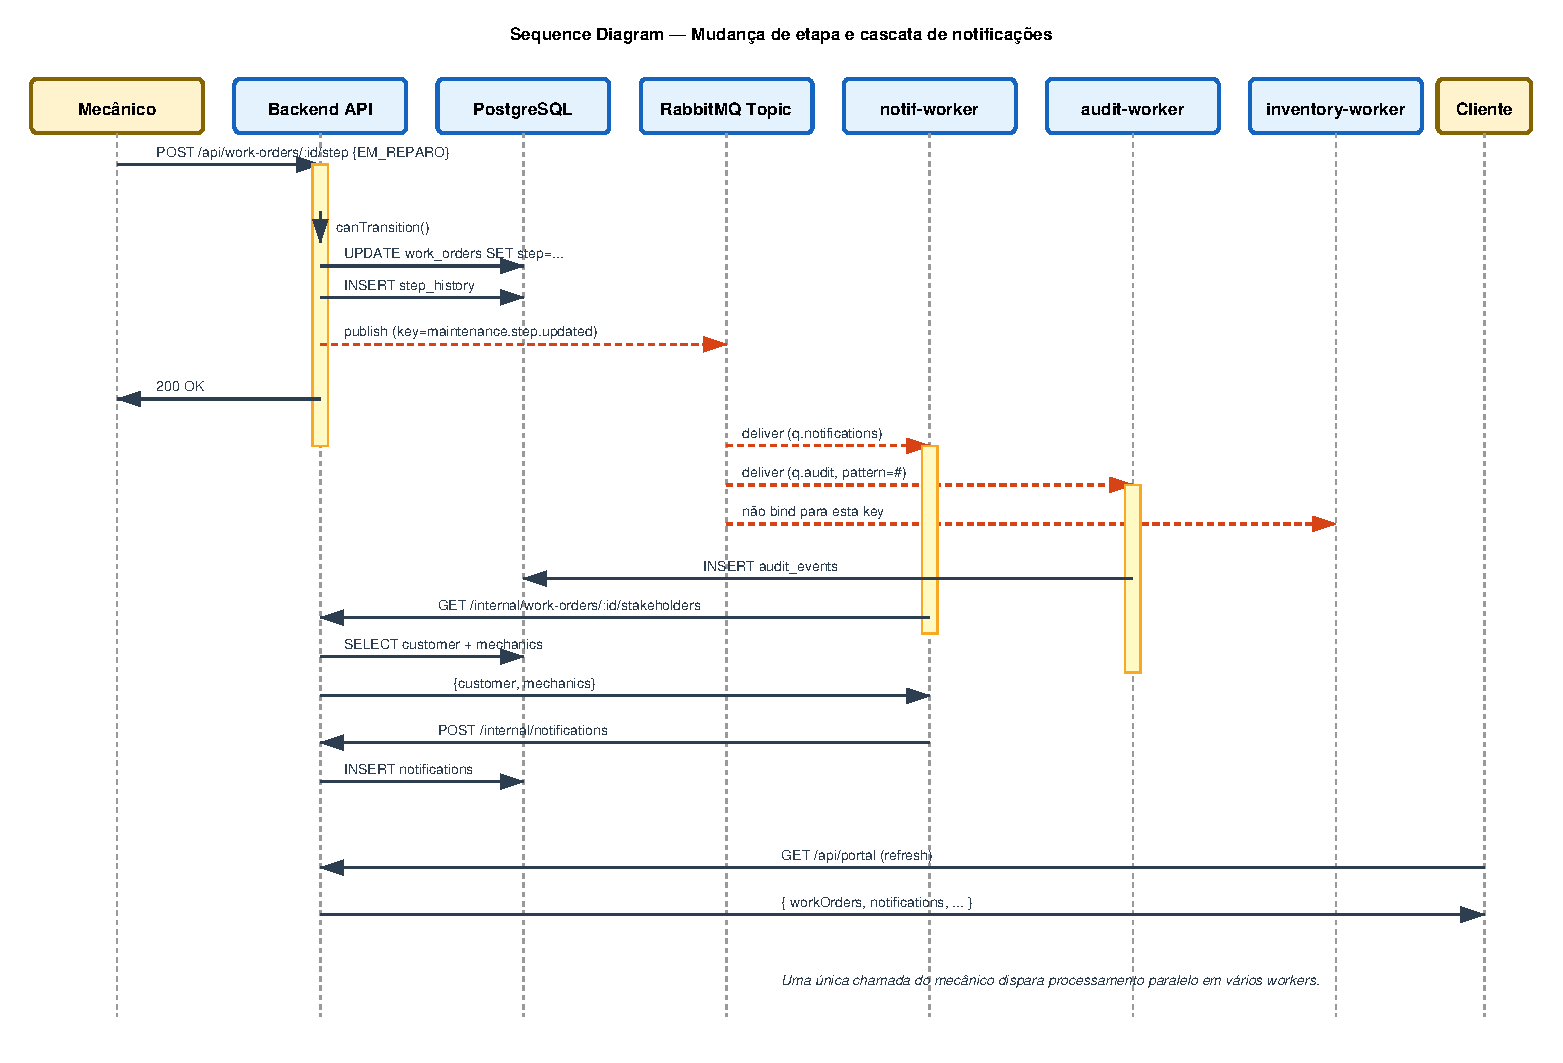
\includegraphics[width=0.72\textwidth]{../diagrams/sequence_etapa.pdf}
\caption{Sequence diagram: mudan\c{c}a de etapa e cascata de notifica\c{c}\~oes.}
\label{fig:seq-etapa}
\end{figure}

\subsubsection*{Implanta\c{c}\~ao h\'\i brida}

A Figura~\ref{fig:deploy} apresenta o diagrama de implanta\c{c}\~ao defendido para produ\c{c}\~ao. Na nuvem, o sistema roda em Kubernetes com pods replicados para frontend e backend, PostgreSQL gerenciado e cluster RabbitMQ de tr\^es n\'os com filas \emph{quorum}. Cada worker tem seu pr\'oprio \emph{deployment} com \emph{Horizontal Pod Autoscaler}. Na borda, a oficina opera com c\^ameras IP, tablets, NAS de 10~TB, mini-broker RabbitMQ federado com o cluster da nuvem e \emph{edge gateway} que funciona offline durante quedas de internet, sincronizando o backlog quando o link \'e restabelecido.

\begin{figure}[H]
\centering
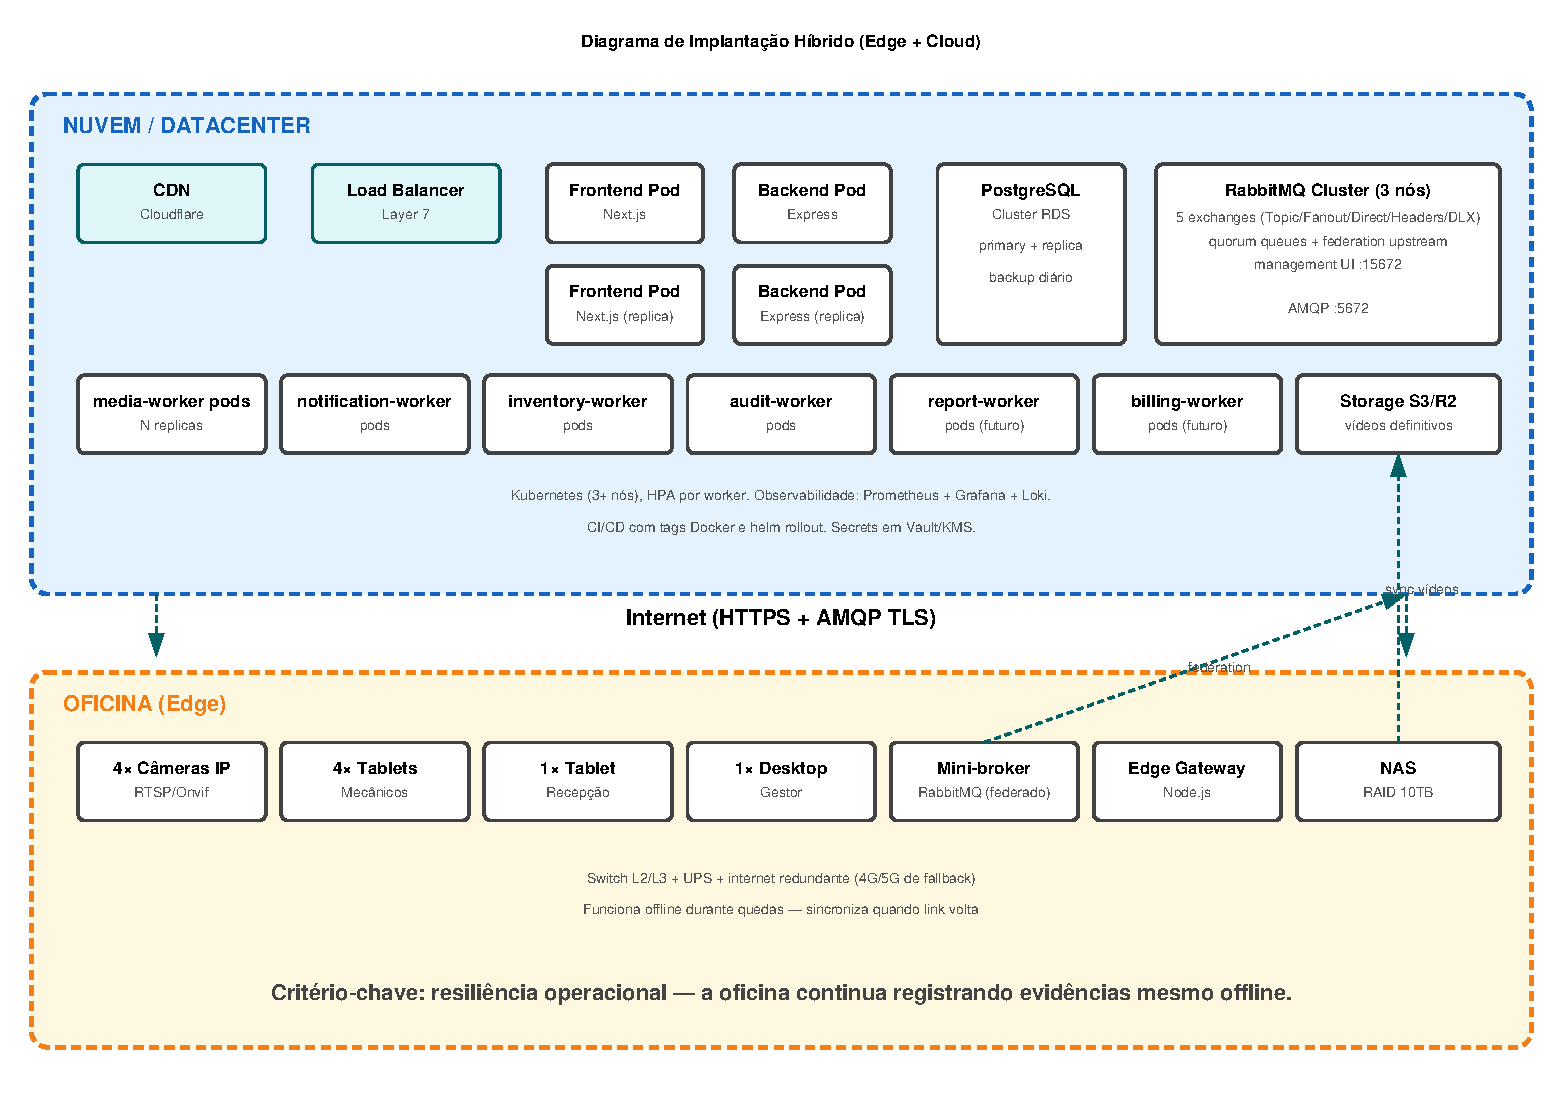
\includegraphics[width=0.72\textwidth]{../diagrams/deployment.pdf}
\caption{Diagrama de implanta\c{c}\~ao h\'\i brido edge + cloud.}
\label{fig:deploy}
\end{figure}

\subsection{Implementa\c{c}\~ao}

O prot\'otipo entregue implementa a fatia central da arquitetura completa: portal web autenticado por papel, backend REST com m\'aquina de estados expl\'\i cita, broker RabbitMQ com cinco exchanges, quatro workers especializados (\texttt{media-worker}, \texttt{notification-worker}, \texttt{inventory-worker}, \texttt{audit-worker}), banco PostgreSQL com nove tabelas e armazenamento local de uploads. Toda a stack \'e empacotada com Docker Compose e sobe com um \'unico comando.

\subsubsection*{Arquitetura t\'ecnica}

O backend (Node.js 20 + Express) exp\~oe rotas REST autenticadas por sess\~ao em mem\'oria e centraliza toda a publica\c{c}\~ao de eventos no m\'odulo \texttt{rabbit.js}. O frontend (Next.js 14, React 18) consome a API via \texttt{fetch}, mantendo o token JWT-like em \texttt{localStorage}. O \texttt{media-worker} processa uploads via a fila \texttt{media.uploaded}; o \texttt{notification-worker} se inscreve em padr\~oes \texttt{maintenance.\#}, \texttt{media.processed}, \texttt{parts.*}, \texttt{budget.*} e \texttt{workorder.\#} no Topic Exchange e cria entradas na tabela \texttt{notifications}; o \texttt{inventory-worker} consome \texttt{parts.requested} e chama o endpoint interno \texttt{/internal/parts/<id>/reserve}; o \texttt{audit-worker} usa o padr\~ao universal ``\texttt{\#}'' e grava todos os eventos na tabela \texttt{audit\_events}.

\subsubsection*{M\'odulos principais}

\paragraph{Camada de mensageria.} O m\'odulo \texttt{backend/src/rabbit.js} (Listing~\ref{lst:rabbit}) declara as cinco exchanges e exp\~oe quatro fun\c{c}\~oes p\'ublicas: \texttt{publishEvent} para o Topic Exchange, \texttt{broadcast} para o Fanout, \texttt{sendCommand} para o Direct, e \texttt{publishNotification} para o Headers Exchange. Cada chamada serializa a mensagem em JSON, marca como \texttt{persistent} e injeta \emph{timestamp}.

\begin{lstlisting}[language=Java,caption={Camada de publica\c{c}\~ao de eventos (resumo)},label=lst:rabbit]
export const EXCHANGES = {
  EVENTS: "oficina.events",         // topic
  BROADCAST: "oficina.broadcast",   // fanout
  COMMANDS: "oficina.commands",     // direct
  NOTIFICATIONS: "oficina.notifications", // headers
  DLX: "oficina.dlx"                // dead letter
};

export async function publishEvent(routingKey, payload, options = {}) {
  const channel = await getChannel();
  const body = Buffer.from(JSON.stringify({
    event: routingKey, timestamp: new Date().toISOString(), ...payload
  }));
  channel.publish(EXCHANGES.EVENTS, routingKey, body, {
    persistent: true, contentType: "application/json", ...options
  });
}
\end{lstlisting}

\paragraph{M\'aquina de estados.} O m\'odulo \texttt{steps.js} declara o conjunto de estados v\'alidos e a tabela de transi\c{c}\~oes permitidas. O controlador \texttt{POST /api/work-orders/:id/step} valida a transi\c{c}\~ao com \texttt{canTransition()} antes de gravar (Listing~\ref{lst:step}). Toda transi\c{c}\~ao bem-sucedida grava no hist\'orico (\texttt{step\_history}) e publica \texttt{maintenance.step.updated} no broker.

\begin{lstlisting}[language=Java,caption={Transi\c{c}\~ao de etapa},label=lst:step]
if (!canTransition(wo.step, newStep)) {
  return res.status(409).json({
    message: `Transicao invalida de ${wo.step} para ${newStep}.`,
    validNext: nextSteps(wo.step)
  });
}
const result = await updateStep(req.params.id, newStep, req.user.id);
await publishEvent(ROUTING_KEYS.STEP_UPDATED, {
  workOrderId: req.params.id,
  fromStep: result.fromStep, toStep: result.toStep,
  changedBy: req.user.id, changedByName: req.user.name
});
\end{lstlisting}

\paragraph{Worker de notifica\c{c}\~oes.} O \texttt{notification-worker} (Listing~\ref{lst:notif}) declara uma fila \texttt{q.notifications} ligada a sete padr\~oes do Topic Exchange. Para cada evento recebido, descobre os \emph{stakeholders} da OS (cliente + mec\^anicos) via endpoint interno e grava notifica\c{c}\~oes personalizadas no banco.

\begin{lstlisting}[language=Java,caption={Notification worker (trecho)},label=lst:notif]
const PATTERNS = [
  "maintenance.step.updated", "media.processed",
  "parts.reserved", "parts.outofstock",
  "budget.created", "budget.approved", "workorder.completed"
];

for (const p of PATTERNS) await ch.bindQueue(QUEUE, EXCHANGE, p);

ch.consume(QUEUE, async (msg) => {
  const payload = JSON.parse(msg.content.toString());
  const rk = msg.fields.routingKey;
  await handle(rk, payload);   // cria notificacao no banco
  ch.ack(msg);
});
\end{lstlisting}

\subsubsection*{Ambiente de execu\c{c}\~ao}

O arquivo \texttt{docker-compose.yml} orquestra sete servi\c{c}os: \texttt{postgres}, \texttt{rabbitmq}, \texttt{backend}, \texttt{media-worker}, \texttt{notification-worker}, \texttt{inventory-worker}, \texttt{audit-worker} e \texttt{frontend}. Os \emph{healthchecks} de Postgres e RabbitMQ controlam a ordem de inicializa\c{c}\~ao. As portas expostas s\~ao 3000 (frontend), 4000 (backend), 5432 (postgres), 5672 (AMQP) e 15672 (RabbitMQ management UI). Subir tudo:
\begin{lstlisting}[language=bash]
$ docker compose up --build
\end{lstlisting}

\section{Avalia\c{c}\~ao do Sistema}

O sistema foi exercitado por meio de quatro cen\'arios end-to-end, executados com a stack levantada em Docker Compose. Os logs do RabbitMQ Management UI foram capturados em \texttt{http://localhost:15672} e os logs dos workers em \texttt{docker compose logs}.

\subsubsection*{Cen\'ario 1 \(textendash\) Mudan\c{c}a de etapa e cascata de notifica\c{c}\~ao}

O mec\^anico ``Maria Souza'' avan\c{c}a a OS \texttt{os-1001} de \texttt{EM\_DIAGNOSTICO} para \texttt{CAUSA\_IDENTIFICADA}. O backend valida a transi\c{c}\~ao, grava em \texttt{step\_history}, e publica \texttt{maintenance.step.updated} na exchange \texttt{oficina.events}. O \texttt{notification-worker} consome a mensagem, descobre que o cliente \'e ``Joao Silva'' e cria a notifica\c{c}\~ao ``Causa identificada''. Simultaneamente, o \texttt{audit-worker} grava o evento na trilha. \textbf{Resultado:} todos os tr\^es processos completam em menos de 500~ms; o cliente, ao atualizar o portal, v\^e a nova notifica\c{c}\~ao e a etapa avan\c{c}ada na linha do tempo.

\subsubsection*{Cen\'ario 2 \(textendash\) Upload de m\'\i dia com processamento ass\'\i ncrono}

O mec\^anico envia tr\^es imagens via endpoint \texttt{POST /api/work-orders/os-1001/media}. O backend grava registros com status \texttt{UPLOADED}, publica tr\^es mensagens \texttt{media.uploaded}, e responde 201 imediatamente. O \texttt{media-worker} consome cada mensagem com \texttt{prefetch=1} (uma de cada vez), aguarda 2~s simulando processamento, e atualiza o status para \texttt{PROCESSED}, publicando \texttt{media.processed}. O \texttt{notification-worker} consome \texttt{media.processed} e gera notifica\c{c}\~oes ``Nova evid\^encia dispon\'\i vel''. \textbf{Resultado:} a API respondeu em $\sim$80~ms, o processamento end-to-end concluiu em $\sim$7~s para tr\^es arquivos, demonstrando o desacoplamento s\'\i ncrono/ass\'\i ncrono.

\subsubsection*{Cen\'ario 3 \(textendash\) Solicita\c{c}\~ao e reserva de pe\c{c}a}

O mec\^anico solicita 4 unidades da pe\c{c}a \texttt{Pastilha de freio dianteira} (\texttt{part-1}, estoque inicial 25). O backend cria a \texttt{part\_request} com status \texttt{PENDING} e publica \texttt{parts.requested}. O \texttt{inventory-worker} consome a mensagem, aguarda 800~ms simulando consulta ao ERP, e chama \texttt{POST /internal/parts/<id>/reserve}. O backend deduz 4 unidades do estoque transaction-ally (com \texttt{SELECT FOR UPDATE}), marca o request como \texttt{RESERVED} e publica \texttt{parts.reserved}. O \texttt{notification-worker} cria a notifica\c{c}\~ao ``Pe\c{c}a reservada'' para o mec\^anico. \textbf{Resultado:} fluxo de tr\^es servi\c{c}os distribu\'\i dos coordenado por eventos, sem chamadas s\'\i ncronas adicionais.

\subsubsection*{Cen\'ario 4 \(textendash\) Auditoria universal}

O \texttt{audit-worker} \'e configurado com \emph{binding pattern} ``\texttt{\#}'' (curinga universal). Ao executar os cen\'arios 1, 2 e 3 em sequ\^encia, foram registrados 11 eventos na tabela \texttt{audit\_events}: \texttt{maintenance.step.updated} (1), \texttt{media.uploaded} (3), \texttt{media.processed} (3), \texttt{parts.requested} (1), \texttt{parts.reserved} (1), e notifica\c{c}\~oes internas (2). \textbf{Resultado:} a trilha de auditoria captura toda a atividade do sistema sem que nenhum c\'odigo a tenha invocado explicitamente \(textendash\) o worker simplesmente assina \texttt{\#}.

\subsubsection*{An\'alise cr\'\i tica}

A solu\c{c}\~ao demonstra de forma concreta os benef\'\i cios da arquitetura orientada a eventos. O backend permanece est\'avel mesmo quando os workers s\~ao reiniciados (as mensagens ficam na fila e s\~ao reentregues). Adicionar um novo worker (por exemplo, um \texttt{report-worker} que ouvisse \texttt{workorder.completed}) n\~ao exige nenhuma altera\c{c}\~ao no backend. A escalabilidade horizontal de cada worker \'e direta: basta subir mais containers do mesmo servi\c{c}o.

As limita\c{c}\~oes do prot\'otipo incluem: (i) sess\~oes mantidas em mem\'oria, o que impede escalar o backend para m\'ultiplas r\'eplicas sem session affinity ou Redis; (ii) processamento de m\'\i dia \'e simulado (n\~ao h\'a FFmpeg real); (iii) o \emph{edge gateway} e a federa\c{c}\~ao RabbitMQ s\~ao apresentados na arquitetura mas n\~ao implementados no prot\'otipo (rodam apenas na nuvem); (iv) o portal n\~ao usa WebSocket ou Server-Sent Events \(textendash\) o cliente atualiza por polling manual; (v) n\~ao h\'a integra\c{c}\~ao real com gateways de e-mail/SMS/WhatsApp.

\subsubsection*{Trabalhos futuros}

Como evolu\c{c}\~oes priorit\'arias: implantar o \emph{edge gateway} real com mini-broker federado; integrar com gateways reais de notifica\c{c}\~ao por Headers Exchange; adicionar push em tempo real via WebSocket; processar m\'\i dia com FFmpeg gerando \emph{thumbnails} e transcodifica\c{c}\~ao; implementar o \texttt{report-worker} para gerar PDF do servi\c{c}o conclu\'\i do; adicionar \emph{quorum queues} para alta disponibilidade do broker; mover armazenamento de v\'\i deos definitivos para S3/R2; adicionar observabilidade com Prometheus e Grafana; implementar \emph{circuit breaker} entre backend e workers; e fechar a integra\c{c}\~ao com sistema fiscal NF-e.

\section{Conclus\~ao}

Este trabalho prop\^os e implementou uma plataforma distribu\'\i da para acompanhamento de manuten\c{c}\~ao veicular, com arquitetura orientada a eventos sobre RabbitMQ. O problema central \(textendash\) a opacidade do servi\c{c}o prestado ao cliente \(textendash\) \'e atacado por meio de uma cadeia de eventos publicados pelo backend a cada a\c{c}\~ao do mec\^anico, consumidos em paralelo por workers especializados em m\'\i dia, notifica\c{c}\~ao, controle de estoque e auditoria. O modelo C4 nos n\'\i veis 1 a 3, a m\'aquina de estados das etapas e os diagramas de sequ\^encia documentam a comunica\c{c}\~ao entre os processos distribu\'\i dos. O prot\'otipo entregue valida a fatia central da arquitetura: cinco exchanges RabbitMQ em uso, quatro workers ativos consumindo padr\~oes de routing distintos, persist\^encia em PostgreSQL, frontend Next.js com controle de acesso por papel, e quatro cen\'arios end-to-end documentados.

Os principais resultados confirmam que o desacoplamento via mensageria fornece a flexibilidade prometida pela teoria: novos workers se conectam sem altera\c{c}\~ao do backend; a falha tempor\'aria de um worker n\~ao bloqueia o fluxo principal; e a trilha de auditoria \'e obtida ``de gra\c{c}a'' por meio de um consumidor inscrito no padr\~ao universal. A principal contribui\c{c}\~ao do trabalho \'e demonstrar \(textendash\) com c\'odigo execut\'avel e cen\'arios reproduz\'\i veis \(textendash\) como cinco padr\~oes de comunica\c{c}\~ao distribu\'\i da (Topic, Fanout, Direct, Headers, DLX) podem ser combinados em um \'unico middleware para resolver um problema concreto de neg\'ocio.

As principais dificuldades enfrentadas foram (i) reconciliar a flexibilidade do Topic Exchange com a necessidade de catalogar e versionar as \emph{routing keys}, (ii) projetar a m\'aquina de estados sem engessar futuras expans\~oes, e (iii) equilibrar a sofistica\c{c}\~ao da arquitetura defendida na apresenta\c{c}\~ao com a fatia que efetivamente couberam no prot\'otipo. Como sugest\~oes futuras destacamos: \emph{quorum queues} para alta disponibilidade, federa\c{c}\~ao real entre broker da oficina e da nuvem, processamento real de m\'\i dia com FFmpeg, integra\c{c}\~ao com gateways de notifica\c{c}\~ao externos por Headers Exchange, observabilidade com Prometheus/Grafana e dashboards de neg\'ocio para o gestor.

\section*{Papeis dos Membros do Grupo}

\begin{tabular}{@{}p{3.5cm}p{3cm}p{8cm}@{}}
\toprule
\textbf{Membro} & \textbf{Papel principal} & \textbf{Contribui\c{c}\~oes} \\
\midrule
Membro~1 & Co-l\'\i der an\'alise & Levantamento bibliogr\'afico e contexto de aplica\c{c}\~ao \\
Membro~2 & An\'alise / Avalia\c{c}\~ao & Requisitos, refer\^encias te\'oricas, cen\'arios de teste, an\'alise cr\'\i tica \\
Membro~3 & Modelagem & Planta da oficina, C4 n\'\i veis 1\(textendash\)3, m\'aquina de estados, sequence diagrams, deployment \\
Membro~4 & Implementa\c{c}\~ao & C\'odigo backend, workers, frontend, ajustes Docker Compose \\
Membro~5 & Avalia\c{c}\~ao & Execu\c{c}\~ao dos cen\'arios, captura de logs, screenshots, an\'alise dos resultados \\
\textbf{Todos} & Consolida\c{c}\~ao & Conclus\~ao, revis\~ao do relat\'orio, slides, apresenta\c{c}\~ao \\
\bottomrule
\end{tabular}

\medskip\noindent\textbf{Reposit\'orio:} \url{https://github.com/<usuario>/projeto-final-sd}

\begin{thebibliography}{9}

\bibitem{tanenbaum2017dist}
A.~S. Tanenbaum and M.~Van Steen, \emph{Distributed Systems: Principles and Paradigms}, 3rd ed. Pearson, 2017.

\bibitem{fowler2017eda}
M.~Fowler, ``What do you mean by `Event-Driven'?,'' \url{https://martinfowler.com/articles/201701-event-driven.html}, 2017.

\bibitem{rabbitmq}
Pivotal/VMware, ``RabbitMQ documentation,'' \url{https://www.rabbitmq.com/documentation.html}, 2024.

\bibitem{kreps2011kafka}
J.~Kreps, N.~Narkhede, and J.~Rao, ``Kafka: A distributed messaging system for log processing,'' in \emph{Proceedings of the NetDB Workshop}, 2011.

\bibitem{eda2020arch}
M.~Richards and N.~Ford, \emph{Fundamentals of Software Architecture}. O'Reilly Media, 2020.

\bibitem{brown2018c4}
S.~Brown, ``The C4 Model for Software Architecture,'' \url{https://c4model.com}, 2018.

\bibitem{hohpe2003eip}
G.~Hohpe and B.~Woolf, \emph{Enterprise Integration Patterns: Designing, Building, and Deploying Messaging Solutions}. Addison-Wesley, 2003.

\bibitem{amqp091}
OASIS, ``AMQP 0-9-1 Protocol Specification,'' \url{https://www.amqp.org/specification/0-9-1/amqp-org-download}, 2008.

\bibitem{edge2020}
W.~Shi, J.~Cao, Q.~Zhang, Y.~Li, and L.~Xu, ``Edge computing: Vision and challenges,'' \emph{IEEE Internet of Things Journal}, vol.~3, no.~5, pp.~637\(textendash\)646, 2016.

\end{thebibliography}

\end{document}